\documentclass[smallextended]{svjour3}
\usepackage[T1]{fontenc}
\usepackage[utf8]{inputenc}
\usepackage{mathptmx}
\usepackage{amsmath,graphicx,booktabs,tabularx,url,placeins}
\usepackage[hidelinks]{hyperref}
\journalname{Computing}
\setlength{\emergencystretch}{2em}
\renewcommand{\thefigure}{S\arabic{figure}}
\renewcommand{\thetable}{S\arabic{table}}
\begin{document}
\title{Online Resource 1: Evaluating Candidate-Restricted Influence Maximization: Reference Budgets, Ranking Precision, and External Topologies}
\titlerunning{Online Resource 1}
\author{Jiayue Sun \and Binbin Yong \and Junjie An \and Tianyu Bo \and Shuai Li}
\institute{Jiayue Sun \at School of Artificial Intelligence, Lanzhou University, Lanzhou 730000, China
\and Binbin Yong (corresponding author) \at School of Information Science and Engineering, Lanzhou University, Lanzhou 730000, China \\
\email{yongbb14@lzu.edu.cn}
\and Junjie An, Tianyu Bo and Shuai Li \at Lanzhou University, Lanzhou, China}
\date{}\maketitle
\paragraph{Scope.} This online resource accompanies the revised manuscript. Tables and figures derive from frozen external outputs. The historical 42-condition study and 520-condition extension are separate evidence layers; the outcome-blind preflight supplies resource measurements only.

\section{Source-scoped related-work comparison}
Table~\ref{tab:related-scope} compares the stated focus of accessible primary
sources, rather than asserting that an item was absent from every implementation
or supplement. ``Not the stated focus'' is not shorthand for ``not done''.
Classical objective/solver work, benchmarking, candidate restriction and learned
inductive estimation address different parts of the influence-maximization
pipeline. This study's contribution is the joint evaluation of reference budget,
ranking precision, coverage, independent utility and cost---not a claim that each
component is individually novel. Complete citations are in the main manuscript.
\begin{table}[htbp]
\caption{Source-scoped comparison of stated evaluation focus. ``Not the stated focus'' does not assert that a feature was absent from every implementation or supplement.}\label{tab:related-scope}
\begin{tabularx}{\linewidth}{p{.19\linewidth}p{.31\linewidth}X}
\toprule
Study & Stated object and role of eligibility & Evaluation dimensions relevant here \\
\midrule
Kempe et al. (2003); CELF/IMM & Expected-spread objective and faster seed selection; fixed full eligibility in the standard formulation & Candidate restriction, held-out utility, cross-budget reference changes, ranking precision and coverage are not the stated comparative object. \\
StaticGreedy (2013) & Reused static realizations for scalable influence maximization & Fixed-world construction is central; this paper does not treat its solver result as evidence about the present restricted-pool evaluation chain. \\
Arora et al. (2017) & Comparative benchmarking of influence-maximization methods & Quality and running-time comparability are relevant; the stated benchmark focus differs from cross-budget evaluation of a fixed truncated ranking. \\
Rui et al. (2020) & Neighbour-scale candidate approach & Candidate restriction and influence outcomes are central; numerical ranking precision and sequence/set-versus-held-out-utility separation are not its stated focus. \\
Ko et al. (2025) & Learned inductive influence estimation/maximization & It changes the estimator and evaluates held-out networks; this differs from preserving a simulator while diagnosing a fixed ranking truncation. \\
This study & Fixed candidate restrictions against finite-world full references & Reports coverage, budget, ranking tolerance, sequence/set agreement, disjoint utility, coupling and scoped costs jointly. \\
\bottomrule
\end{tabularx}
\end{table}


\section{Audit and reproducibility}
Figures~\ref{fig:matrix}--\ref{fig:loss-cost} provide the full default-budget
comparison, the direction diagnostic and the descriptive loss--cost analysis,
complementing the main-text evaluation framework, budget--precision comparison
and independent reference-transition plot.

There are 54 configuration-defined external conditions and 468 executed arms.
The archive retains one JSON and NPZ pair per condition, source and data manifests,
world-ID hashes, candidate IDs, selected sequences, all round/candidate integer
totals and 10,000 evaluation values per arm. Reproduction checks the raw gzip
hashes before using the frozen runner. The independent audit
parses topology, checks all recorded hashes and world IDs, reconstructs all
argmax/tie decisions, replays every full-candidate score matrix and all evaluation
arrays, and checks a scalar Python oracle on the first 16 worlds for each
distinct ordered selection within a graph/path/coupling. Complete replay and the
independent sampled oracle are different validation layers.

Frozen source files are unchanged. The original runner's entry checks did not
enforce actual raw hashes against the data manifest; the retrospective comparison
and new guarded wrapper address that enforcement gap without rewriting history.
ca-GrQc removes loops before collecting endpoints: raw vertex 12295 appears only
in a loop, explaining 5,241 rather than 5,242 vertices. The original prose was
ambiguous about endpoint collection order, while the processed size/hash were
already frozen before outcomes. Results refer to that processed graph.

Direction is part of the simulation definition. CollegeMsg goes from sender to
receiver; wiki-Vote from voter to votee; ca-GrQc uses reciprocal arcs. The first
two are directed observed relations, not measured causal diffusion. PageRank uses
standard incoming importance, while the objective follows outgoing propagation.
Direction diagnostics are post-hoc and do not isolate a causal mechanism.

\subsection{Preprocessing and evidence provenance}
CollegeMsg retains the first $\lfloor .65T\rfloor$ complete timestamp groups,
where $T=58,911$, through Unix timestamp 1085640224, yielding 38,939 non-self
messages. The processed CollegeMsg, ca-GrQc and wiki-Vote graphs have 2, 354 and
24 weak components. Every retained component is included. The later CollegeMsg
events are not held-out influence cascades. The ca-GrQc size and hash were
recorded before outcomes; reinserting its self-loop-only vertex would change
lexical indices and hashed draws, so the 5,241-node representation defines the
reported experiment.

The initial historical study contains 42 conditions and 168 arms, two paths,
$W=20,80,320$ and $M=2000$. Its separate extension contains 520 conditions and
4,680 arms, ten paths on four real contact graphs, selection budgets up to 5120
and $M=10,000$. The four contact graphs contain 91, 212, 402 and 75 vertices;
two synthetic controls contain 2,000 vertices each. Synthetic topology weights
are not independent historical-event evidence. Local protocol freezes are not
public preregistrations. External resource preflight used $W=80,320$ and
$M=1000$ without examining selected seeds or utilities; it supplies resource
measurements only.

\subsection{Finite-world coupling counterexample}
Consider the chain $s\to u\to v$ with horizon two. In one step-indexed world,
$s\to u$ is open at step zero, while $u\to v$ is closed at step zero and open
at step one. Starting with $\{s\}$ reaches all three vertices. Starting with
$\{s,u\}$ activates $u$ earlier and reaches only two. Thus the finite-world
objective is not necessarily monotone, even though the marginal law for each
fixed seed set remains the intended independent-cascade law. This example alone
does not establish a violation of submodularity. The fixed-edge control instead
uses horizon-limited reachability in each sampled graph, giving a monotone,
submodular coverage objective. Both implementations enumerate all eligible
vertices at every round. The external world-ID audit checks 169,200 distinct
identifiers across graph, path and selection/evaluation families for collisions.

\section{Statistical interpretation}
For a fixed selected pair, conditional Monte Carlo standard error is the sample
standard deviation of 10,000 paired per-world differences divided by 100.
Normal intervals are pointwise and conditional. Across-path SD describes five
computational paths, or three control paths, and includes finite evaluation noise.
The optional $t$ intervals in CSVs are post-hoc descriptive intervals, not
population-of-network inference. Random pools are averaged within each path
before cross-path analysis; their shared-world covariance is retained.

Incremental spread subtracts five seeds from total spread. Percentage loss is
minus the paired mean difference divided by full incremental spread, times 100.
The plug-in percentage does not have a guaranteed loss-bound interpretation.
The primary sign-test family is three methods within each graph at $W=1280$.
All nonzero PageRank and random-mean differences are negative, but five paths
limit the minimum two-sided exact sign-test value to .0625. Nonsignificance is
not equivalence. Table~\ref{tab:tests} reports all nine tests without exclusions.

\section{Cost and repeated measurements}
The archived preparation timer contains parsing, all rankings, hashes and graph
diagnostics. Its ranking subtimers are not added to it again. A separate
post-hoc setup study measures five repetitions of raw parsing/CSR and one
method's ranking plus pool generation. The frozen selection timer already includes
lexical candidate sorting; it is not charged again. Hybrid deployment cost adds that
median setup to frozen selection-world preparation and selection. Hybrid
verification cost adds independent-world preparation and independent evaluation.
These are assembled warm-process, cached-file estimates, not direct end-to-end
trials. Imports, JIT compilation, downloads and output writing are excluded.

Frozen repeated timing uses path 1101 and $W=320$, five randomized repetitions
per arm, yielding 130 observations. Selected sequences and per-world evaluations
were required to remain identical. The CSVs report every repetition and its
selection/evaluation time, plus medians and ranges. The maximum positive psutil
process-lifetime peak is 3.448822 GiB; it must not be confused with an unverified
PowerShell display or with preflight measurements using one tenth the evaluation
world count. Timings are machine- and implementation-specific.

\section{Complete aggregate results}
Tables~\ref{tab:s-ca_grqc}--\ref{tab:s-wiki_vote} retain every method at all external
budgets/couplings. Total spread, paired difference, between-path SD, percentage
incremental loss and ordered agreement are shown. CSVs additionally retain
candidate fractions, set agreement, Jaccard, first divergence, conditional
uncertainty, costs and every path. This avoids treating an averaged random seed
set as if it existed. There were no failed or excluded main conditions.
\begin{table}[htbp]
\caption{Prespecified primary exact two-sided sign tests at $W=1280$. Holm correction is across three methods within each fixed graph. Zero path differences are dropped from the sign test.}\label{tab:tests}
\begin{tabular}{llrrrr}
\toprule
Graph & Method & Mean $\Delta$ & Zeros & $p$ & Holm $p$ \\
\midrule
CollegeMsg & Degree 4k & 0.00000 & 5 & 1.0000 & 1.0000 \\
CollegeMsg & PageRank 4k & -0.90780 & 0 & 0.0625 & 0.1875 \\
CollegeMsg & Random mean & -8.22745 & 0 & 0.0625 & 0.1875 \\
ca-GrQc & Degree 4k & 0.00000 & 5 & 1.0000 & 1.0000 \\
ca-GrQc & PageRank 4k & -0.25082 & 0 & 0.0625 & 0.1875 \\
ca-GrQc & Random mean & -3.94366 & 0 & 0.0625 & 0.1875 \\
wiki-Vote & Degree 4k & 0.00000 & 5 & 1.0000 & 1.0000 \\
wiki-Vote & PageRank 4k & -40.69334 & 0 & 0.0625 & 0.1875 \\
wiki-Vote & Random mean & -50.90179 & 0 & 0.0625 & 0.1875 \\
\bottomrule
\end{tabular}
\end{table}

\begin{table}[htbp]
\caption{ca-GrQc: complete frozen aggregate matrix; PageRank uses default tolerance. E means fixed-edge coupling (three paths); other rows use five step-coupled paths. SD is across path mean differences. Random pools are averaged within each path; their agreement entry is a fraction.}\label{tab:s-ca_grqc}
\begin{tabular}{rlrrrrr}
\toprule
$W$ & Method & Total & $\Delta$ & SD & Loss (\%) & Order \\
\midrule
80 & Degree 4k & 9.636 & +0.226 & 0.190 & -5.16 & 1/5 \\
80 & Degree 5\% & 9.410 & +0.000 & 0.000 & 0.00 & 5/5 \\
80 & Full & 9.410 & +0.000 & 0.000 & 0.00 & 5/5 \\
80 & PageRank 4k & 9.646 & +0.236 & 0.274 & -5.61 & 0/5 \\
80 & PageRank 5\% & 9.522 & +0.111 & 0.125 & -2.62 & 2/5 \\
80 & Random mean & 5.961 & -3.449 & 0.303 & 78.14 & 0.00 \\
320 & Degree 4k & 9.845 & +0.038 & 0.086 & -0.83 & 4/5 \\
320 & Degree 5\% & 9.806 & +0.000 & 0.000 & 0.00 & 5/5 \\
320 & Full & 9.806 & +0.000 & 0.000 & 0.00 & 5/5 \\
320 & PageRank 4k & 9.680 & -0.126 & 0.181 & 2.53 & 0/5 \\
320 & PageRank 5\% & 9.806 & +0.000 & 0.000 & 0.00 & 5/5 \\
320 & Random mean & 5.983 & -3.824 & 0.272 & 79.50 & 0.00 \\
1280 & Degree 4k & 9.934 & +0.000 & 0.000 & 0.00 & 5/5 \\
1280 & Degree 5\% & 9.934 & +0.000 & 0.000 & 0.00 & 5/5 \\
1280 & Full & 9.934 & +0.000 & 0.000 & 0.00 & 5/5 \\
1280 & PageRank 4k & 9.683 & -0.251 & 0.076 & 5.07 & 0/5 \\
1280 & PageRank 5\% & 9.934 & +0.000 & 0.000 & 0.00 & 5/5 \\
1280 & Random mean & 5.990 & -3.944 & 0.221 & 79.90 & 0.00 \\
320E & Degree 4k & 9.934 & +0.082 & 0.079 & -1.70 & 1/3 \\
320E & Degree 5\% & 9.852 & +0.000 & 0.000 & 0.00 & 3/3 \\
320E & Full & 9.852 & +0.000 & 0.000 & 0.00 & 3/3 \\
320E & PageRank 4k & 9.689 & -0.162 & 0.086 & 3.33 & 0/3 \\
320E & PageRank 5\% & 9.904 & +0.052 & 0.090 & -1.09 & 2/3 \\
320E & Random mean & 6.108 & -3.744 & 0.137 & 77.16 & 0.00 \\
\bottomrule
\end{tabular}
\end{table}

\begin{table}[htbp]
\caption{CollegeMsg: complete frozen aggregate matrix; PageRank uses default tolerance. E means fixed-edge coupling (three paths); other rows use five step-coupled paths. SD is across path mean differences. Random pools are averaged within each path; their agreement entry is a fraction.}\label{tab:s-college_msg}
\begin{tabular}{rlrrrrr}
\toprule
$W$ & Method & Total & $\Delta$ & SD & Loss (\%) & Order \\
\midrule
80 & Degree 4k & 14.919 & +0.000 & 0.000 & 0.00 & 5/5 \\
80 & Degree 5\% & 14.919 & +0.000 & 0.000 & 0.00 & 5/5 \\
80 & Full & 14.919 & +0.000 & 0.000 & 0.00 & 5/5 \\
80 & History 4k & 14.597 & -0.322 & 0.229 & 3.21 & 0/5 \\
80 & History 5\% & 14.919 & +0.000 & 0.000 & 0.00 & 5/5 \\
80 & PageRank 4k & 13.991 & -0.928 & 0.295 & 9.33 & 0/5 \\
80 & PageRank 5\% & 14.461 & -0.457 & 0.297 & 4.57 & 0/5 \\
80 & Random mean & 6.804 & -8.114 & 0.146 & 81.84 & 0.00 \\
320 & Degree 4k & 15.019 & +0.000 & 0.000 & 0.00 & 5/5 \\
320 & Degree 5\% & 15.019 & +0.000 & 0.000 & 0.00 & 5/5 \\
320 & Full & 15.019 & +0.000 & 0.000 & 0.00 & 5/5 \\
320 & History 4k & 14.820 & -0.199 & 0.130 & 1.97 & 0/5 \\
320 & History 5\% & 15.019 & +0.000 & 0.000 & 0.00 & 5/5 \\
320 & PageRank 4k & 14.164 & -0.854 & 0.117 & 8.52 & 0/5 \\
320 & PageRank 5\% & 14.645 & -0.374 & 0.125 & 3.72 & 0/5 \\
320 & Random mean & 6.836 & -8.183 & 0.211 & 81.70 & 0.00 \\
1280 & Degree 4k & 15.072 & +0.000 & 0.000 & 0.00 & 5/5 \\
1280 & Degree 5\% & 15.072 & +0.000 & 0.000 & 0.00 & 5/5 \\
1280 & Full & 15.072 & +0.000 & 0.000 & 0.00 & 5/5 \\
1280 & History 4k & 14.820 & -0.252 & 0.024 & 2.50 & 0/5 \\
1280 & History 5\% & 15.072 & +0.000 & 0.000 & 0.00 & 5/5 \\
1280 & PageRank 4k & 14.164 & -0.908 & 0.041 & 9.01 & 0/5 \\
1280 & PageRank 5\% & 14.641 & -0.431 & 0.043 & 4.28 & 0/5 \\
1280 & Random mean & 6.845 & -8.227 & 0.266 & 81.69 & 0.00 \\
320E & Degree 4k & 15.062 & +0.000 & 0.000 & 0.00 & 3/3 \\
320E & Degree 5\% & 15.062 & +0.000 & 0.000 & 0.00 & 3/3 \\
320E & Full & 15.062 & +0.000 & 0.000 & 0.00 & 3/3 \\
320E & History 4k & 14.790 & -0.272 & 0.037 & 2.71 & 0/3 \\
320E & History 5\% & 15.062 & +0.000 & 0.000 & 0.00 & 3/3 \\
320E & PageRank 4k & 14.128 & -0.934 & 0.031 & 9.28 & 0/3 \\
320E & PageRank 5\% & 14.631 & -0.431 & 0.046 & 4.28 & 0/3 \\
320E & Random mean & 6.925 & -8.137 & 0.293 & 80.87 & 0.00 \\
\bottomrule
\end{tabular}
\end{table}

\begin{table}[htbp]
\caption{wiki-Vote: complete frozen aggregate matrix; PageRank uses default tolerance. E means fixed-edge coupling (three paths); other rows use five step-coupled paths. SD is across path mean differences. Random pools are averaged within each path; their agreement entry is a fraction.}\label{tab:s-wiki_vote}
\begin{tabular}{rlrrrrr}
\toprule
$W$ & Method & Total & $\Delta$ & SD & Loss (\%) & Order \\
\midrule
80 & Degree 4k & 60.736 & +0.000 & 0.000 & 0.00 & 5/5 \\
80 & Degree 5\% & 60.736 & +0.000 & 0.000 & 0.00 & 5/5 \\
80 & Full & 60.736 & +0.000 & 0.000 & 0.00 & 5/5 \\
80 & PageRank 4k & 20.043 & -40.693 & 0.138 & 73.01 & 0/5 \\
80 & PageRank 5\% & 46.855 & -13.882 & 0.107 & 24.91 & 0/5 \\
80 & Random mean & 9.775 & -50.961 & 1.921 & 91.43 & 0.00 \\
320 & Degree 4k & 60.736 & +0.000 & 0.000 & 0.00 & 5/5 \\
320 & Degree 5\% & 60.736 & +0.000 & 0.000 & 0.00 & 5/5 \\
320 & Full & 60.736 & +0.000 & 0.000 & 0.00 & 5/5 \\
320 & PageRank 4k & 20.014 & -40.722 & 0.112 & 73.06 & 0/5 \\
320 & PageRank 5\% & 46.986 & -13.750 & 0.250 & 24.67 & 0/5 \\
320 & Random mean & 9.831 & -50.905 & 1.897 & 91.33 & 0.00 \\
1280 & Degree 4k & 60.736 & +0.000 & 0.000 & 0.00 & 5/5 \\
1280 & Degree 5\% & 60.736 & +0.000 & 0.000 & 0.00 & 5/5 \\
1280 & Full & 60.736 & +0.000 & 0.000 & 0.00 & 5/5 \\
1280 & PageRank 4k & 20.043 & -40.693 & 0.138 & 73.01 & 0/5 \\
1280 & PageRank 5\% & 47.206 & -13.530 & 0.096 & 24.28 & 0/5 \\
1280 & Random mean & 9.834 & -50.902 & 1.892 & 91.33 & 0.00 \\
320E & Degree 4k & 60.663 & +0.000 & 0.000 & 0.00 & 3/3 \\
320E & Degree 5\% & 60.663 & +0.000 & 0.000 & 0.00 & 3/3 \\
320E & Full & 60.663 & +0.000 & 0.000 & 0.00 & 3/3 \\
320E & PageRank 4k & 20.087 & -40.576 & 0.003 & 72.90 & 0/3 \\
320E & PageRank 5\% & 47.050 & -13.613 & 0.209 & 24.46 & 0/3 \\
320E & Random mean & 9.394 & -51.269 & 1.963 & 92.11 & 0.00 \\
\bottomrule
\end{tabular}
\end{table}

\begin{figure}[htbp]
\centering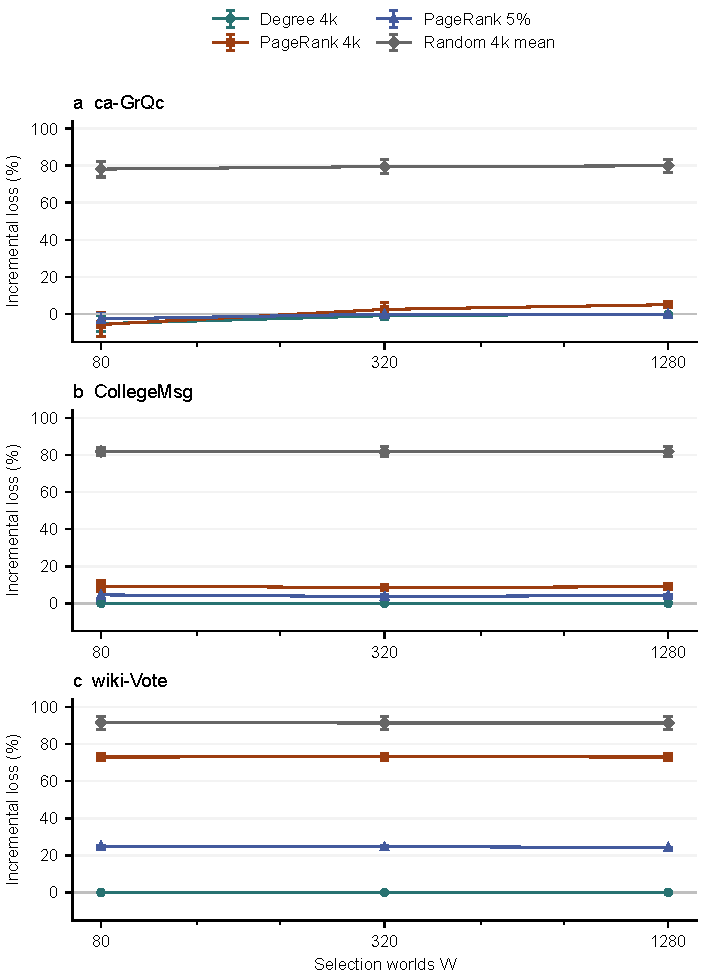
\includegraphics[width=\linewidth]{Fig1.pdf}
\caption{Complete default-tolerance budget comparison. Points are mean incremental
losses over five paths; bars are path standard deviations. Random-pool repeats
are averaged within each path. Negative loss denotes independently evaluated
gain against the finite reference; all graph panels use a common percentage
scale.}\label{fig:matrix}
\end{figure}
\section{Post-hoc PageRank precision control}
The frozen default tolerance is $10^{-6}$, and NetworkX stops on a successive
vector $L_1$ change below $n$ times that value. A candidate-only diagnostic at
$10^{-12}$ changed some pool members on ca-GrQc and wiki-Vote; pools agreed
between $10^{-12}$ and $10^{-14}$. Before inspecting new utility outputs, a
separate protocol froze two PageRank arms on every graph and all five original
$W=1280$ paths. Its 15 conditions and 30 arms are a numerical sensitivity control,
not independent confirmation and not additional paths in the primary tests.

Table~\ref{tab:precision} shows that tightening tolerance changes ca-GrQc's 4k
mean difference from $-0.25082$ to $+0.02608$, replacing all five selected sets.
Its original small loss is therefore not precision-robust. CollegeMsg outcomes
are unchanged. wiki-Vote's 4k loss remains large ($-41.21970$, or 73.96\% of
incremental spread), and its 5\% loss is 24.47\%. This diagnostic qualifies the
ranking interpretation without replacing any original observation or retroactively
redefining the frozen sign-test family. Tightened-solver timing is not substituted
into the default-solver cost curves.
\begin{table}[htbp]
\caption{Post-hoc precision control at $W=1280$, tolerance $10^{-12}$. Difference is versus frozen full greedy; change is versus the default PageRank implementation. Order compares with default PageRank, not full eligibility. These are the original five paths, not new independent samples.}\label{tab:precision}
\begin{tabular}{llrrrr}
\toprule
Graph & Pool & Difference & Loss (\%) & Change & Order \\
\midrule
ca-GrQc & PageRank 4k & 0.02608 & -0.54 & +0.27690 & 0/5 \\
ca-GrQc & PageRank 5\% & 0.00000 & 0.00 & +0.00000 & 5/5 \\
CollegeMsg & PageRank 4k & -0.90780 & 9.01 & +0.00000 & 5/5 \\
CollegeMsg & PageRank 5\% & -0.43094 & 4.28 & +0.00000 & 5/5 \\
wiki-Vote & PageRank 4k & -41.21970 & 73.96 & -0.52636 & 0/5 \\
wiki-Vote & PageRank 5\% & -13.63982 & 24.47 & -0.10970 & 3/5 \\
\bottomrule
\end{tabular}
\end{table}

\section{Post-hoc precision--budget control}
The initial precision control left a material question open because it covered
only $W=1280$. A new protocol was frozen before new utility outputs were inspected
and added strict PageRank-4k and PageRank-5\% arms at $W=80,320$ for all three
graphs and five original paths. It contributes 30 conditions and 60 restricted
arms, reusing the frozen full references and disjoint evaluation-world IDs. Together
with the prior strict $W=1280$ layer, this is a 45-condition, 90-arm post-hoc
sensitivity study; it adds no independent paths or primary tests.

Strict $10^{-12}$ pools agree with $10^{-14}$ pools for every graph/pool size.
CollegeMsg's strict and default pools are identical. ca-GrQc changes two of 20
4k candidates (pool Jaccard .818), while wiki-Vote changes one (Jaccard .905).
The lower-budget results show that ca-GrQc's default PageRank-4k direction reversal
does not survive the stable strict pool: strict losses are -11.25\%, -2.96\% and
-0.54\% at $W=80,320,1280$. Its selected sets and paired utility magnitude still
change with budget. CollegeMsg retains 9.33\%, 8.52\% and 9.01\% strict 4k losses;
wiki-Vote retains 74.05\%, 74.05\% and 73.96\%. These are graph-specific,
post-hoc sensitivity findings, not an equivalence, superiority or significance claim.
\begin{table}[htbp]
\caption{Post-hoc PageRank loss across budgets. Each entry is the mean incremental-loss percentage across five original paths at $W=80/320/1280$. Default uses NetworkX tolerance $10^{-6}$; strict uses $10^{-12}$, whose pool is unchanged at $10^{-14}$. Pool Jaccard compares default and strict candidates. This is a numerical sensitivity analysis, not a new primary test family.}\label{tab:precision-budget}
\begin{tabular}{llrrr}
\toprule
Graph & Pool & Default loss (\%) & Strict loss (\%) & Pool Jaccard \\
\midrule
ca-GrQc & 4k & -5.61 / 2.53 / 5.07 & -11.25 / -2.96 / -0.54 & 0.818 \\
ca-GrQc & 5\% & -2.62 / 0.00 / 0.00 & -2.62 / 0.00 / 0.00 & 0.977 \\
CollegeMsg & 4k & 9.33 / 8.52 / 9.01 & 9.33 / 8.52 / 9.01 & 1.000 \\
CollegeMsg & 5\% & 4.57 / 3.72 / 4.28 & 4.57 / 3.72 / 4.28 & 1.000 \\
wiki-Vote & 4k & 73.01 / 73.06 / 73.01 & 74.05 / 74.05 / 73.96 & 0.905 \\
wiki-Vote & 5\% & 24.91 / 24.67 / 24.28 & 24.83 / 24.67 / 24.47 & 0.994 \\
\bottomrule
\end{tabular}
\end{table}

\section{Coverage, direction and reference transitions}
The direction illustration in Fig.~\ref{fig:direction-detail} supports a
graph-specific interpretation of wiki-Vote's loss. At $W=1280$, path 1101 gives
the full seed set $\{2565,766,11,457,2688\}$.
The PageRank-4k set is $\{3352,2237,2328,2654,1297\}$.
The same final sets occur on all five paths.
The PageRank pool contains none of the full-reference seeds. Its mean incremental
spread is 15.04268 nodes, compared with 55.73602 for full selection, a paired
difference of $-40.69334$ nodes. These coverage facts are consistent with a
mismatch between incoming importance and outgoing propagation; without a
direction intervention they do not establish causality.
\begin{figure}[htbp]
\centering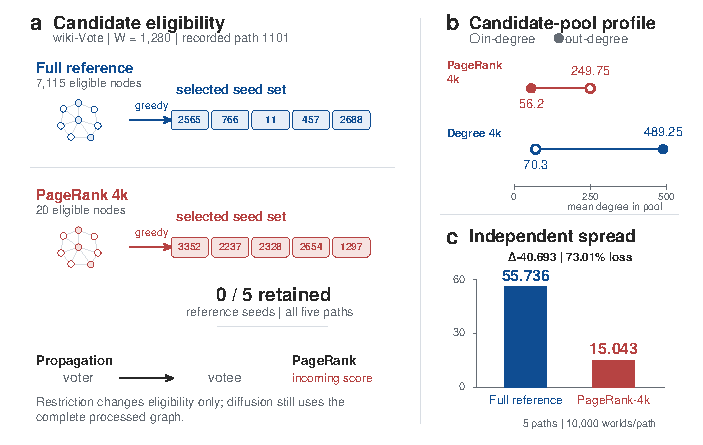
\includegraphics[width=\linewidth]{FigDirectionMechanism.pdf}
\caption{Post-hoc direction and candidate-coverage diagnostic for wiki-Vote.
The illustrated seed sets, stored voter-to-votee orientation and independent
spread values connect candidate eligibility to the measured loss at $W=1280$.
The diagram describes this graph and propagation convention.}\label{fig:direction-detail}
\end{figure}
Table~\ref{tab:transitions} supplies the aggregate reference-transition values
underlying the main-text paired spread plot. Identical final sets have identical
evaluation vectors and hence exactly zero paired differences.
\begin{table}[htbp]
\caption{Full-reference transitions under step coupling. Gain is the paired independent change in total spread; seed counts are constant. The range is across paths, not a confidence interval.}\label{tab:transitions}
\begin{tabular}{llrrr}
\toprule
Graph & Budgets & Set changed & Mean gain & Path range \\
\midrule
ca-GrQc & 80--320 & 5/5 & +0.39616 & +0.1819, +0.6139 \\
ca-GrQc & 320--1280 & 5/5 & +0.12720 & -0.0266, +0.2411 \\
CollegeMsg & 80--320 & 2/5 & +0.09994 & +0.0000, +0.2855 \\
CollegeMsg & 320--1280 & 1/5 & +0.05336 & +0.0000, +0.2668 \\
wiki-Vote & 80--320 & 0/5 & +0.00000 & +0.0000, +0.0000 \\
wiki-Vote & 320--1280 & 0/5 & +0.00000 & +0.0000, +0.0000 \\
\bottomrule
\end{tabular}
\end{table}


\section{Descriptive utility--cost thresholds}
Figure~\ref{fig:loss-cost} retains all frozen loss thresholds. Degree-4k meets
zero point-estimate loss on every highest-budget path. Default PageRank-4k meets
10\% on ca-GrQc and CollegeMsg, but not 20\% on wiki-Vote. The 5\% PageRank
pool meets zero loss on ca-GrQc and 5\% on CollegeMsg, and still fails 20\% on
wiki-Vote. No within-path random-pool mean meets 20\%. These thresholds are
descriptive; no application-specific acceptable loss or noninferiority margin
is inferred. Strict-tolerance timing is not substituted into this analysis.
\begin{figure}[htbp]
\centering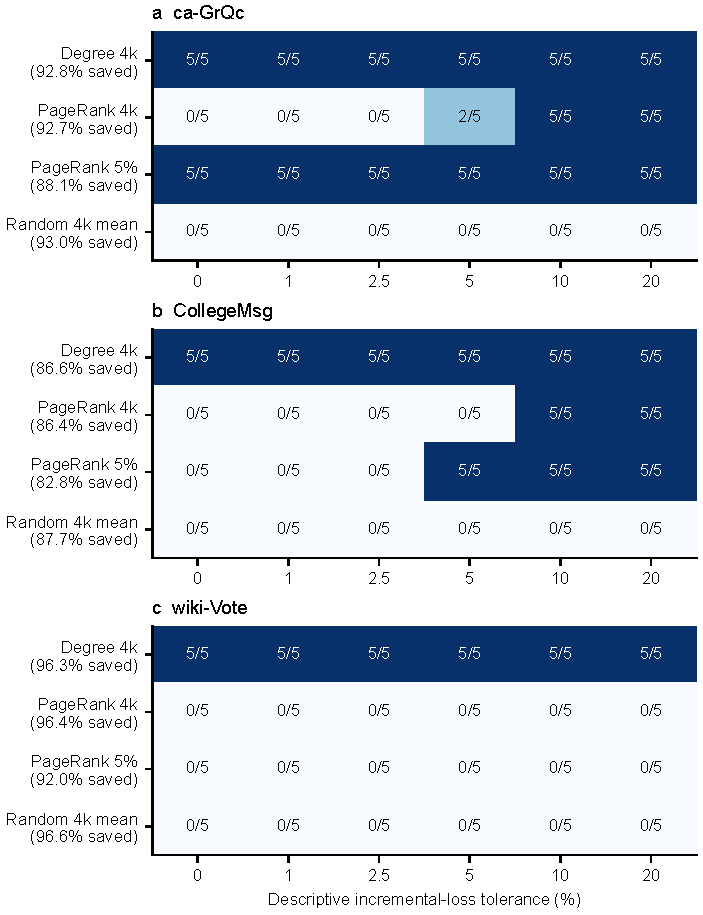
\includegraphics[width=\linewidth]{Fig3.pdf}
\caption{Loss--cost decisions for default tolerance at $W=1280$. Cells count
paths with point-estimate incremental loss at or below the column threshold.
Row labels show mean assembled verification-inclusive savings across all five
paths. Random rows average three pools within each path and use the mean cost
of one random-pool deployment.}\label{fig:loss-cost}
\end{figure}
\section{Coupling control}
Figure~\ref{fig:coupling} shows all preselected W320 control paths for the main
ranking comparisons. Mean PageRank-4k differences under edge coupling are
$-0.16240$, $-0.93417$ and $-40.57597$ on ca-GrQc, CollegeMsg and wiki-Vote.
Degree-4k ordered agreement is 1/3, 3/3 and 3/3, respectively. This control
preserves the prominent PageRank losses while showing that coupling can change
reference reproduction. It does not estimate a general coupling-invariance law.
\begin{figure}[htbp]
\centering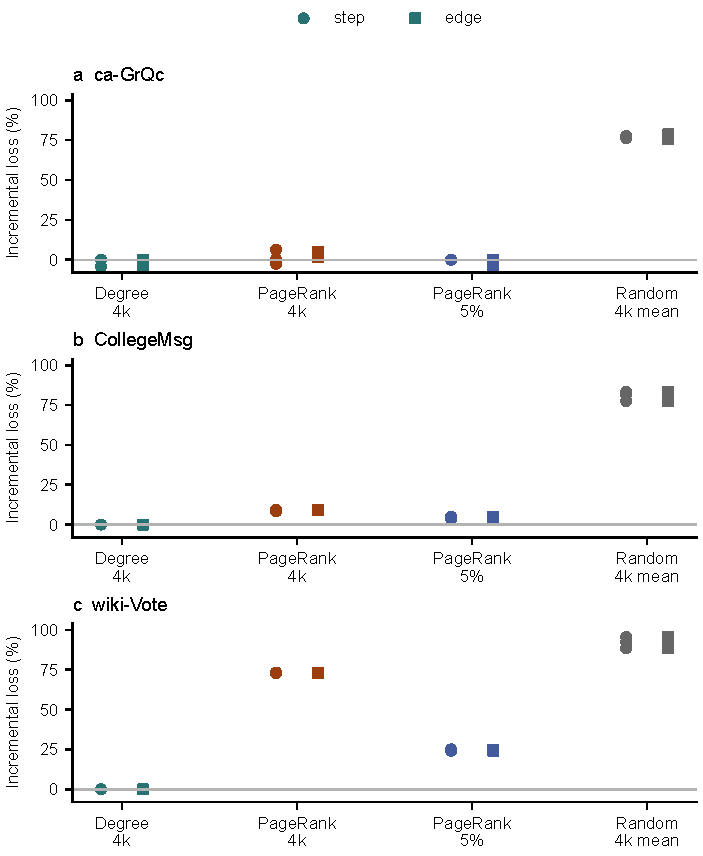
\includegraphics[width=\linewidth]{FigS1.pdf}
\caption{Coupling control at $W=320$. Each symbol is one of three preselected
computational paths, with three random-pool repetitions first averaged within
path. Circles denote step-indexed worlds and squares fixed-edge worlds. Loss is
relative to the full reference using the same coupling. No inferential intervals
are implied by these point displays}\label{fig:coupling}
\end{figure}
\section{File map and availability}
The reproducibility package supplied with the submission contains frozen configuration, source and data manifests;
all 54 result pairs; the strict audit; per-path and summary statistics; plotting
scripts and source CSVs; manuscript sources and PDFs; the novelty/evaluation
summary; a cover-letter draft; an author checklist; and environment/reproduction
instructions. A separate historical-evidence directory preserves the previous
extension and its analysis rather than merging the evidence layers.

The guarded download script obtains public sources only after checking their
expected hashes. Raw third-party archives are not redistributed. No public
archive URL is asserted. The package is supplied for editorial and peer-review
access with the manuscript.
\end{document}
